\documentclass[]{article}
\usepackage{lmodern}
\usepackage{amssymb,amsmath}
\usepackage{ifxetex,ifluatex}
\usepackage{fixltx2e} % provides \textsubscript
\ifnum 0\ifxetex 1\fi\ifluatex 1\fi=0 % if pdftex
  \usepackage[T1]{fontenc}
  \usepackage[utf8]{inputenc}
\else % if luatex or xelatex
  \ifxetex
    \usepackage{mathspec}
  \else
    \usepackage{fontspec}
  \fi
  \defaultfontfeatures{Ligatures=TeX,Scale=MatchLowercase}
\fi
% use upquote if available, for straight quotes in verbatim environments
\IfFileExists{upquote.sty}{\usepackage{upquote}}{}
% use microtype if available
\IfFileExists{microtype.sty}{%
\usepackage{microtype}
\UseMicrotypeSet[protrusion]{basicmath} % disable protrusion for tt fonts
}{}
\usepackage[margin=1in]{geometry}
\usepackage{hyperref}
\hypersetup{unicode=true,
            pdftitle={Thesis Reports},
            pdfauthor={S.Dehbod},
            pdfborder={0 0 0},
            breaklinks=true}
\urlstyle{same}  % don't use monospace font for urls
\usepackage{graphicx,grffile}
\makeatletter
\def\maxwidth{\ifdim\Gin@nat@width>\linewidth\linewidth\else\Gin@nat@width\fi}
\def\maxheight{\ifdim\Gin@nat@height>\textheight\textheight\else\Gin@nat@height\fi}
\makeatother
% Scale images if necessary, so that they will not overflow the page
% margins by default, and it is still possible to overwrite the defaults
% using explicit options in \includegraphics[width, height, ...]{}
\setkeys{Gin}{width=\maxwidth,height=\maxheight,keepaspectratio}
\IfFileExists{parskip.sty}{%
\usepackage{parskip}
}{% else
\setlength{\parindent}{0pt}
\setlength{\parskip}{6pt plus 2pt minus 1pt}
}
\setlength{\emergencystretch}{3em}  % prevent overfull lines
\providecommand{\tightlist}{%
  \setlength{\itemsep}{0pt}\setlength{\parskip}{0pt}}
\setcounter{secnumdepth}{0}
% Redefines (sub)paragraphs to behave more like sections
\ifx\paragraph\undefined\else
\let\oldparagraph\paragraph
\renewcommand{\paragraph}[1]{\oldparagraph{#1}\mbox{}}
\fi
\ifx\subparagraph\undefined\else
\let\oldsubparagraph\subparagraph
\renewcommand{\subparagraph}[1]{\oldsubparagraph{#1}\mbox{}}
\fi

%%% Use protect on footnotes to avoid problems with footnotes in titles
\let\rmarkdownfootnote\footnote%
\def\footnote{\protect\rmarkdownfootnote}

%%% Change title format to be more compact
\usepackage{titling}

% Create subtitle command for use in maketitle
\newcommand{\subtitle}[1]{
  \posttitle{
    \begin{center}\large#1\end{center}
    }
}

\setlength{\droptitle}{-2em}

  \title{Thesis Reports}
    \pretitle{\vspace{\droptitle}\centering\huge}
  \posttitle{\par}
    \author{S.Dehbod}
    \preauthor{\centering\large\emph}
  \postauthor{\par}
      \predate{\centering\large\emph}
  \postdate{\par}
    \date{January 8, 2019}

\usepackage{booktabs}
\usepackage{longtable}
\usepackage{array}
\usepackage{multirow}
\usepackage[table]{xcolor}
\usepackage{wrapfig}
\usepackage{float}
\usepackage{colortbl}
\usepackage{pdflscape}
\usepackage{tabu}
\usepackage{threeparttable}
\usepackage{threeparttablex}
\usepackage[normalem]{ulem}
\usepackage{makecell}

\begin{document}
\maketitle

\section{\texorpdfstring{For \(\alpha\) = 2, p(reduced dimention) =
2}{For \textbackslash{}alpha = 2, p(reduced dimention) = 2}}\label{for-alpha-2-preduced-dimention-2}

\subsection{Tabel\_A2D2}\label{tabel_a2d2}

\begin{table}[H]
\centering\rowcolors{2}{gray!6}{white}

\begin{tabular}{lrrr}
\hiderowcolors
\toprule
Dataset & ARI\_d & ARI\_p & C\_e\\
\midrule
\showrowcolors
Thyroid & 0.5831656 & 0.3989981 & -18\\
Iris & 0.6201352 & 0.4710315 & -15\\
Diabetes & 0.3801662 & 0.3647537 & -2\\
Swiss Banknotes & 0.8456292 & 0.3880871 & -46\\
Seeds & 0.7732937 & 0.4482112 & -33\\
\addlinespace
Crabs & 0.0481402 & 0.0439549 & 0\\
Mice Protein Expression & 0.1316117 & 0.0657659 & -7\\
\bottomrule
\end{tabular}
\rowcolors{2}{white}{white}
\end{table}

\subsection{Histograms}\label{histograms}

\begin{center}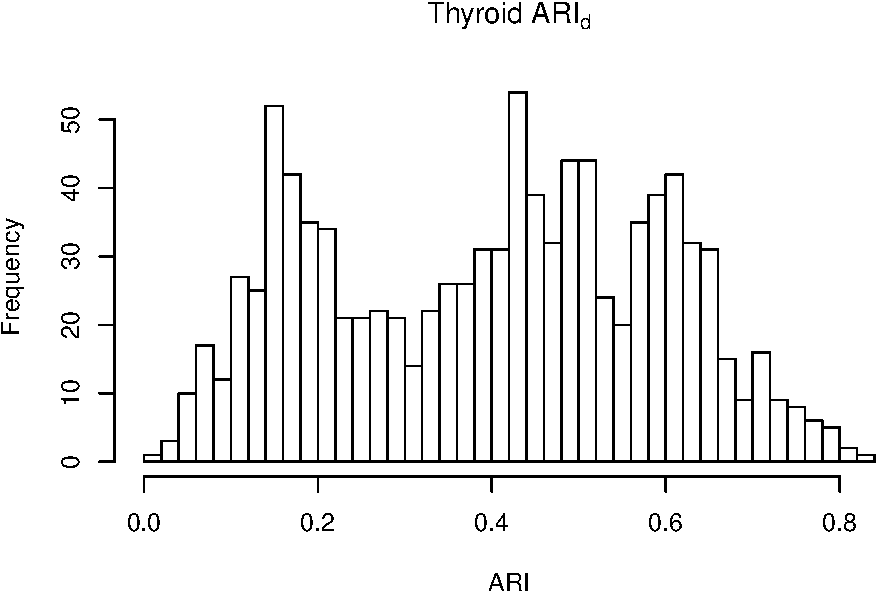
\includegraphics[width=1\linewidth]{Report_files/figure-latex/unnamed-chunk-3-1} \end{center}

\begin{center}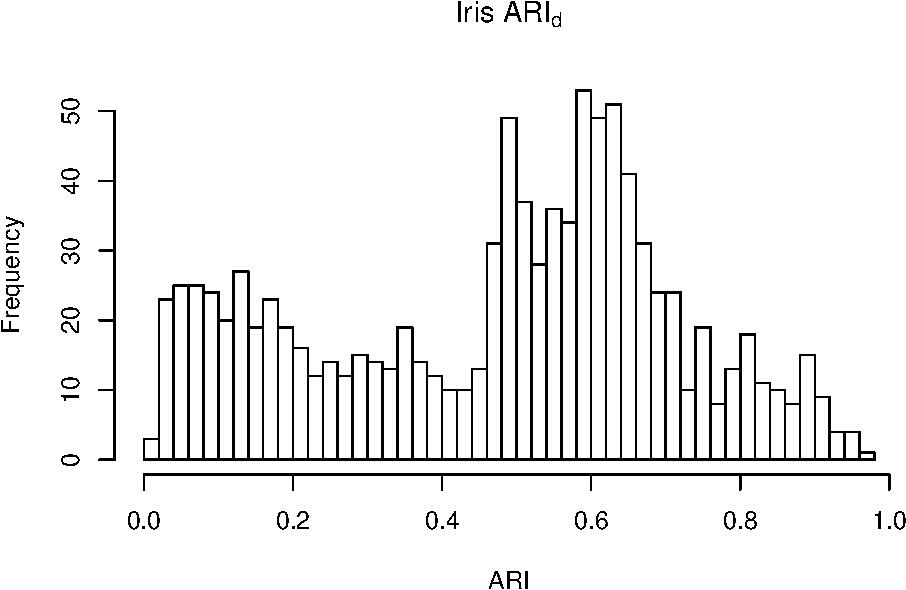
\includegraphics[width=1\linewidth]{Report_files/figure-latex/unnamed-chunk-3-2} \end{center}

\begin{center}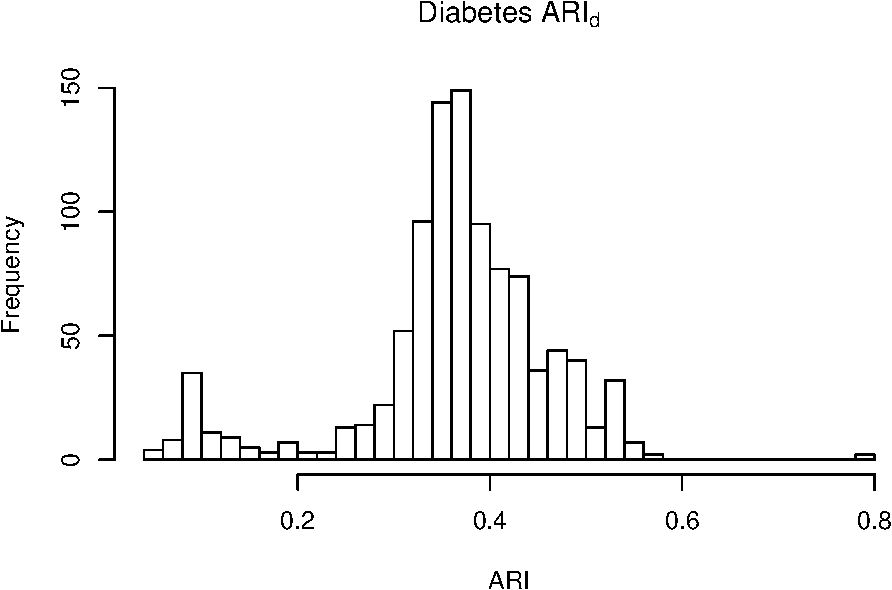
\includegraphics[width=1\linewidth]{Report_files/figure-latex/unnamed-chunk-3-3} \end{center}

\begin{center}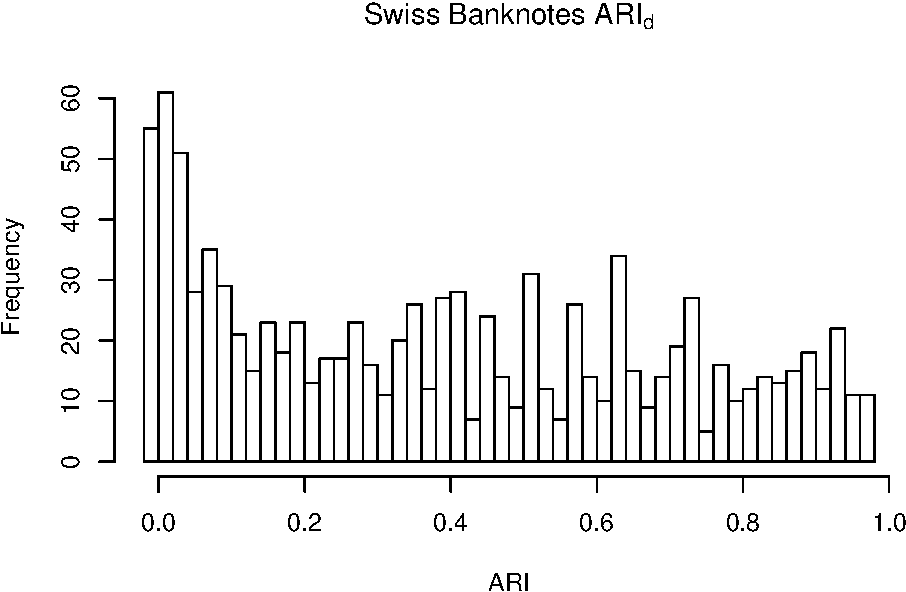
\includegraphics[width=1\linewidth]{Report_files/figure-latex/unnamed-chunk-3-4} \end{center}

\begin{center}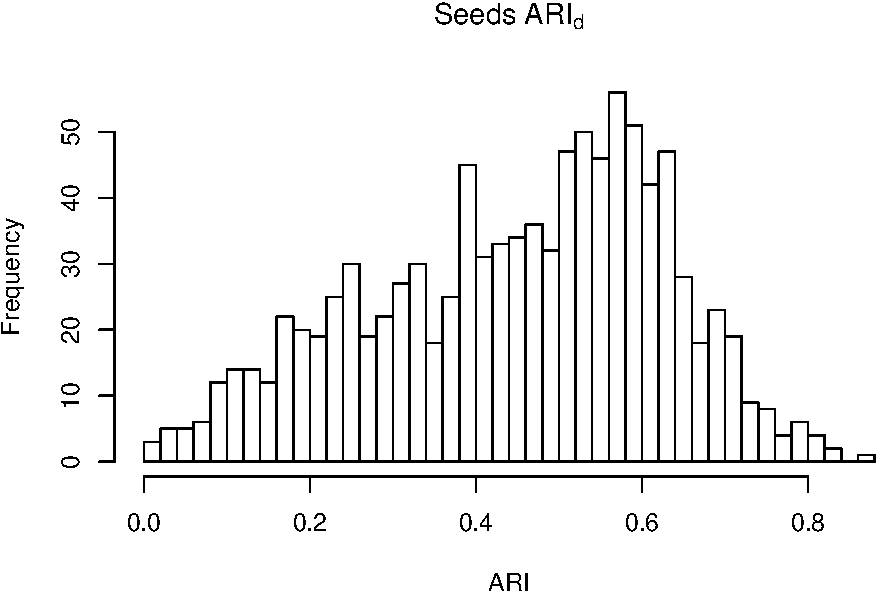
\includegraphics[width=1\linewidth]{Report_files/figure-latex/unnamed-chunk-3-5} \end{center}

\begin{center}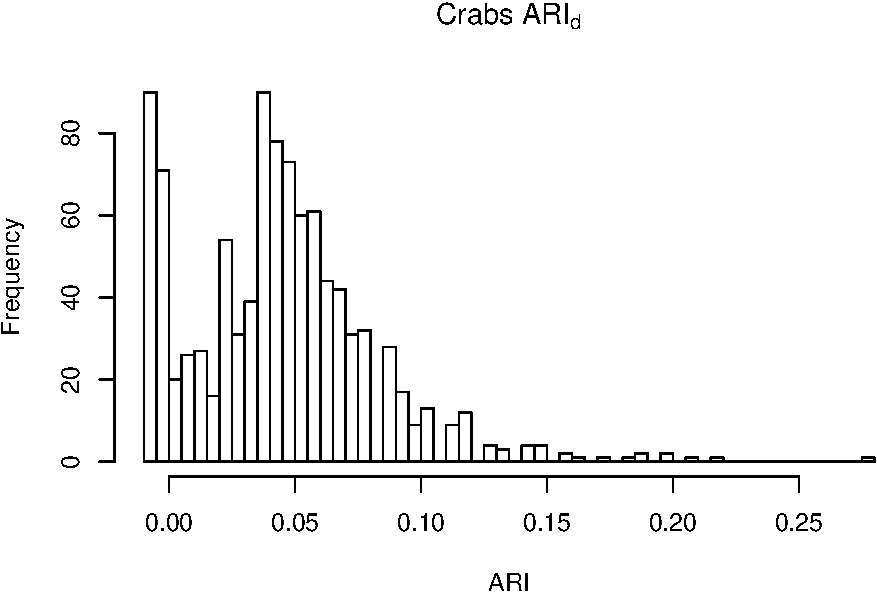
\includegraphics[width=1\linewidth]{Report_files/figure-latex/unnamed-chunk-3-6} \end{center}

\begin{center}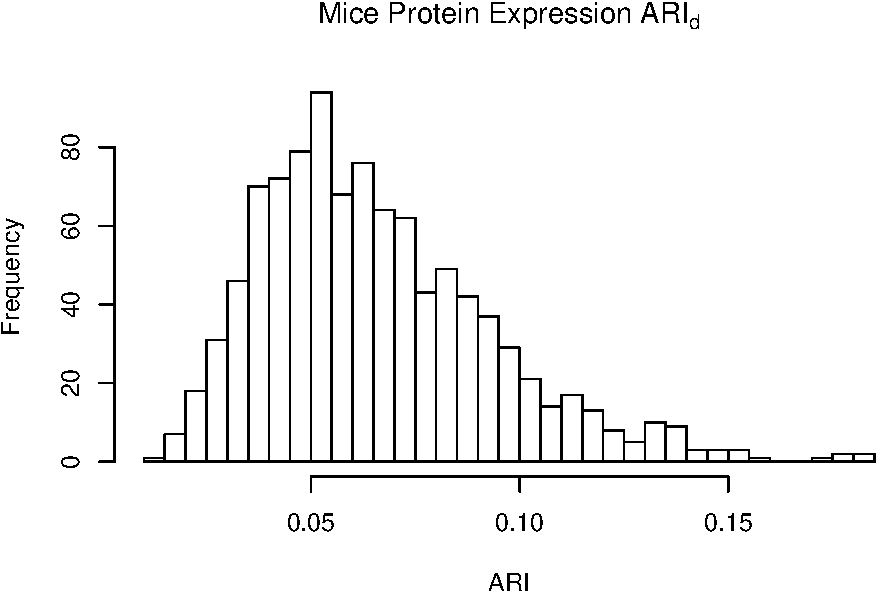
\includegraphics[width=1\linewidth]{Report_files/figure-latex/unnamed-chunk-3-7} \end{center}

\section{\texorpdfstring{For \(\alpha\) = 2, p(reduced dimention) =
3}{For \textbackslash{}alpha = 2, p(reduced dimention) = 3}}\label{for-alpha-2-preduced-dimention-3}

\subsection{Tabel}\label{tabel}

\begin{table}[H]
\centering\rowcolors{2}{gray!6}{white}

\begin{tabular}{lrrr}
\hiderowcolors
\toprule
Dataset & ARI\_d & ARI\_p & C\_e\\
\midrule
\showrowcolors
Thyroid & 0.5831656 & 0.4344288 & -15\\
Iris & 0.6201352 & 0.5359746 & -8\\
Diabetes & 0.3801662 & 0.3805076 & 0\\
Swiss Banknotes & 0.8456292 & 0.4714675 & -37\\
Seeds & 0.7732937 & 0.5299329 & -24\\
\addlinespace
Mice Protein Expression & 0.1316575 & 0.0814613 & -5\\
Crabs & 0.0481402 & 0.0485252 & 0\\
\bottomrule
\end{tabular}
\rowcolors{2}{white}{white}
\end{table}

\subsection{Histograms}\label{histograms-1}

\begin{center}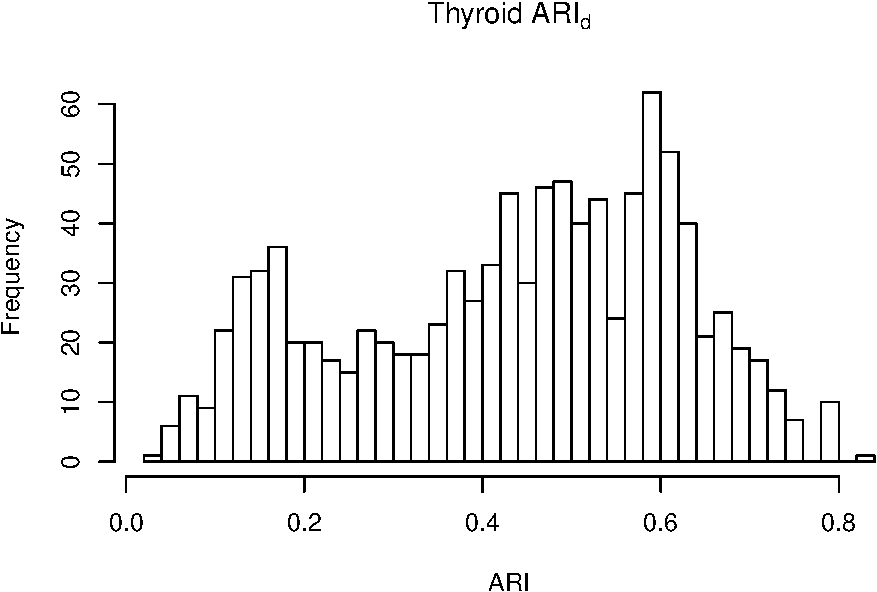
\includegraphics[width=1\linewidth]{Report_files/figure-latex/unnamed-chunk-6-1} \end{center}

\begin{center}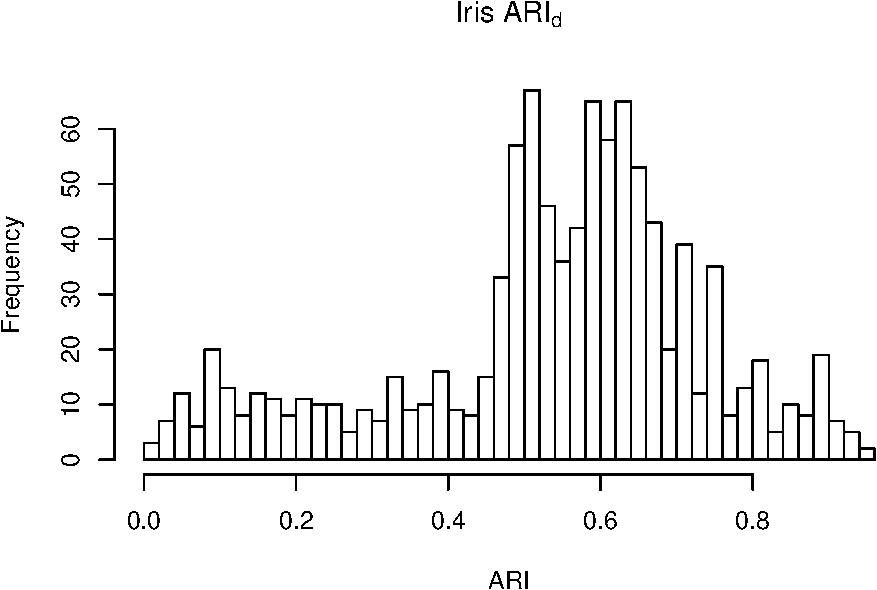
\includegraphics[width=1\linewidth]{Report_files/figure-latex/unnamed-chunk-6-2} \end{center}

\begin{center}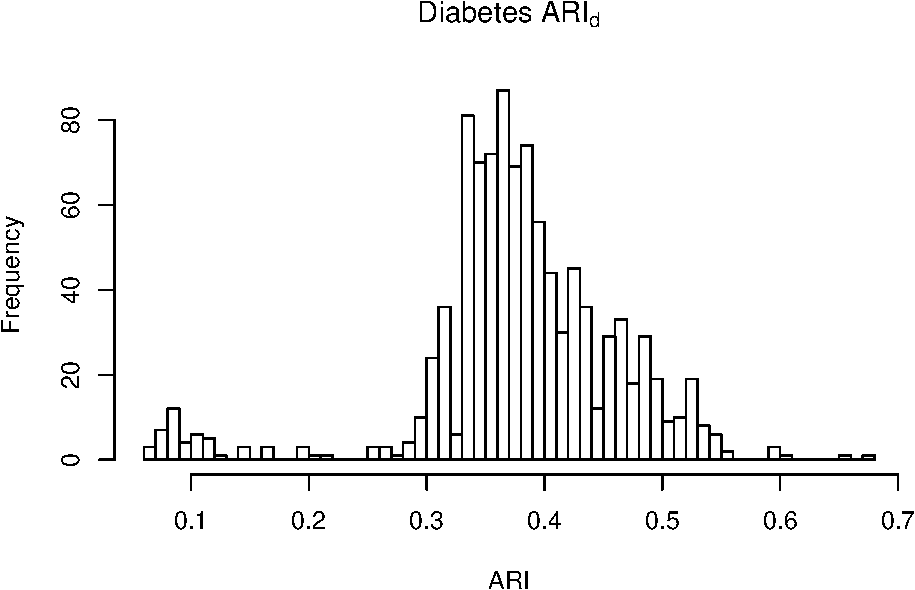
\includegraphics[width=1\linewidth]{Report_files/figure-latex/unnamed-chunk-6-3} \end{center}

\begin{center}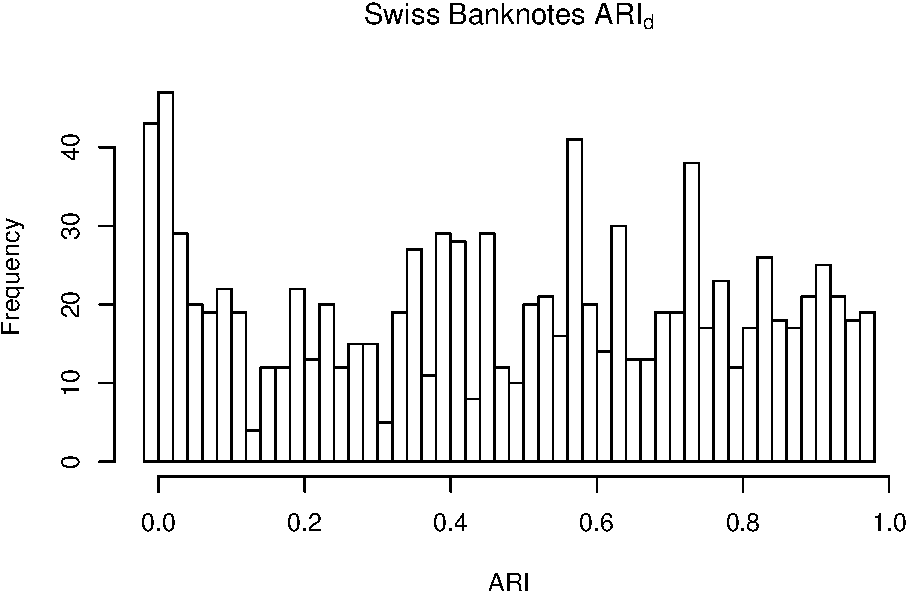
\includegraphics[width=1\linewidth]{Report_files/figure-latex/unnamed-chunk-6-4} \end{center}

\begin{center}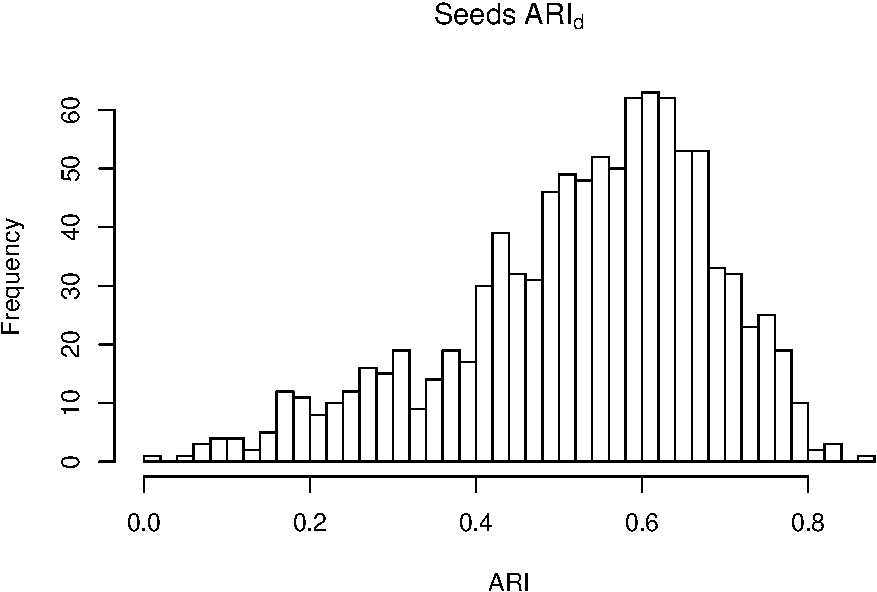
\includegraphics[width=1\linewidth]{Report_files/figure-latex/unnamed-chunk-6-5} \end{center}

\begin{center}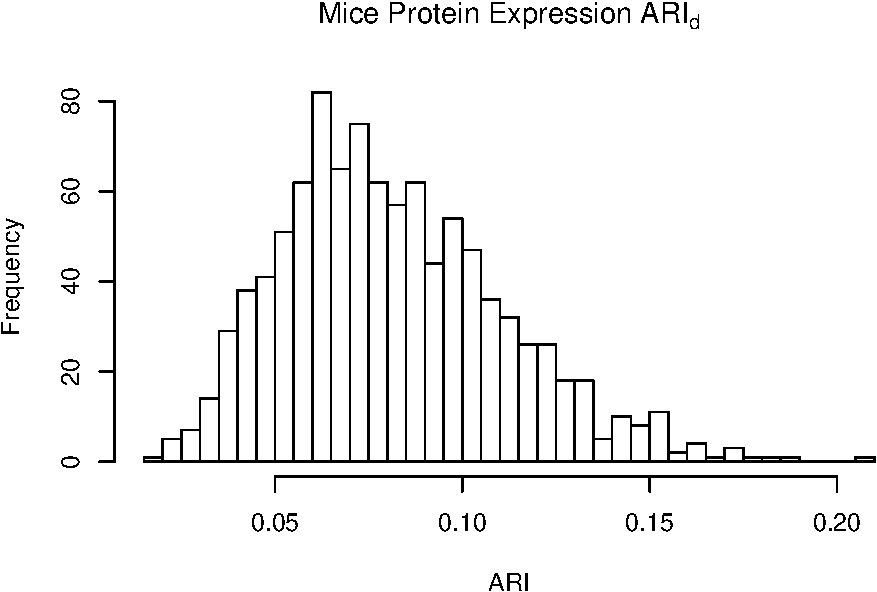
\includegraphics[width=1\linewidth]{Report_files/figure-latex/unnamed-chunk-6-6} \end{center}

\begin{center}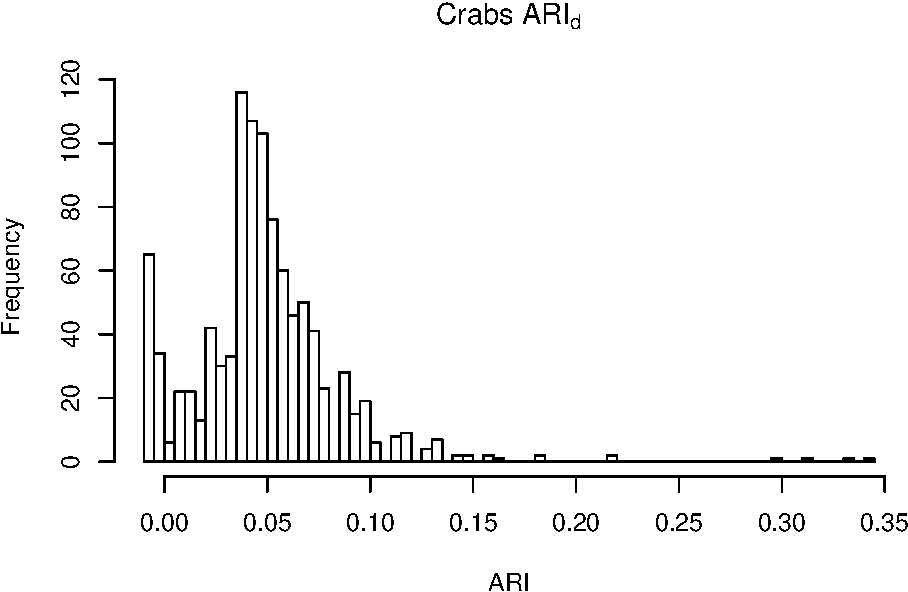
\includegraphics[width=1\linewidth]{Report_files/figure-latex/unnamed-chunk-6-7} \end{center}

\section{\texorpdfstring{For \(\alpha\) = 1, p(reduced dimention) =
2}{For \textbackslash{}alpha = 1, p(reduced dimention) = 2}}\label{for-alpha-1-preduced-dimention-2}

\subsection{Tabel}\label{tabel-1}

\begin{table}[H]
\centering\rowcolors{2}{gray!6}{white}

\begin{tabular}{lrrr}
\hiderowcolors
\toprule
Dataset & ARI\_d & ARI\_p & C\_e\\
\midrule
\showrowcolors
Thyroid & 0.5831656 & 0.3559301 & -23\\
Iris & 0.6201352 & 0.5078172 & -11\\
Diabetes & 0.3801662 & 0.3341399 & -5\\
Swiss Banknotes & 0.8456292 & 0.4011119 & -44\\
Seeds & 0.7732937 & 0.4488349 & -32\\
\addlinespace
Mice Protein Expression & 0.1317342 & 0.0592468 & -7\\
Crabs & 0.0481402 & 0.0469365 & 0\\
\bottomrule
\end{tabular}
\rowcolors{2}{white}{white}
\end{table}

\subsection{Histograms}\label{histograms-2}

\begin{center}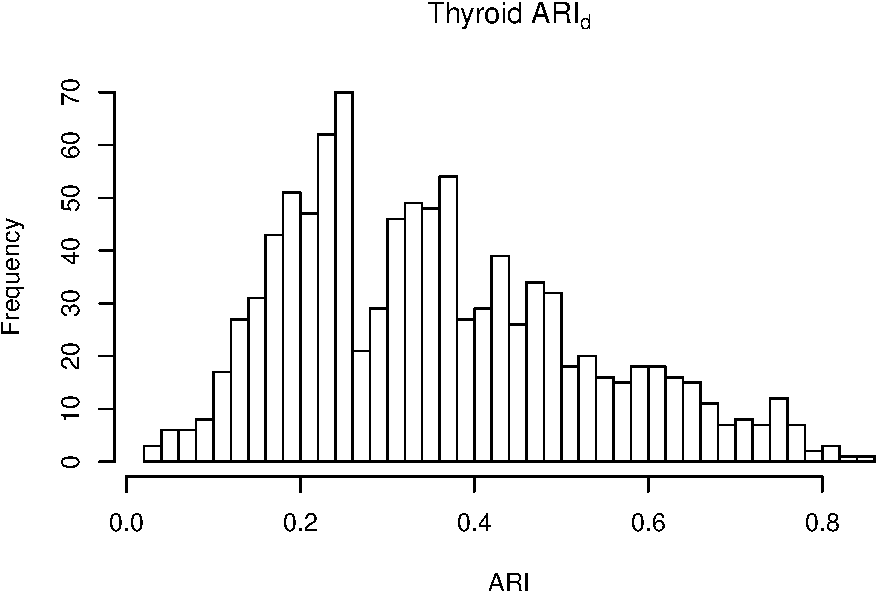
\includegraphics[width=1\linewidth]{Report_files/figure-latex/unnamed-chunk-9-1} \end{center}

\begin{center}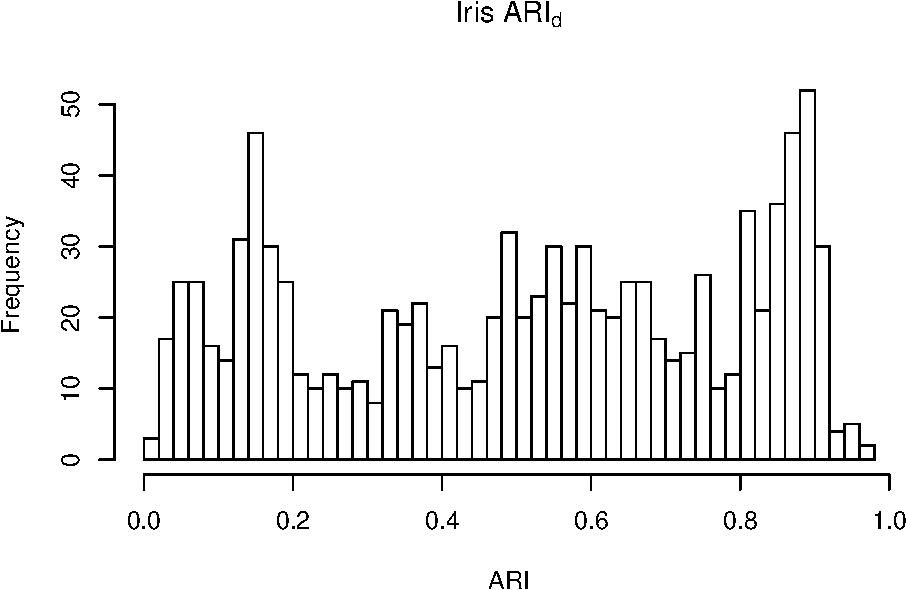
\includegraphics[width=1\linewidth]{Report_files/figure-latex/unnamed-chunk-9-2} \end{center}

\begin{center}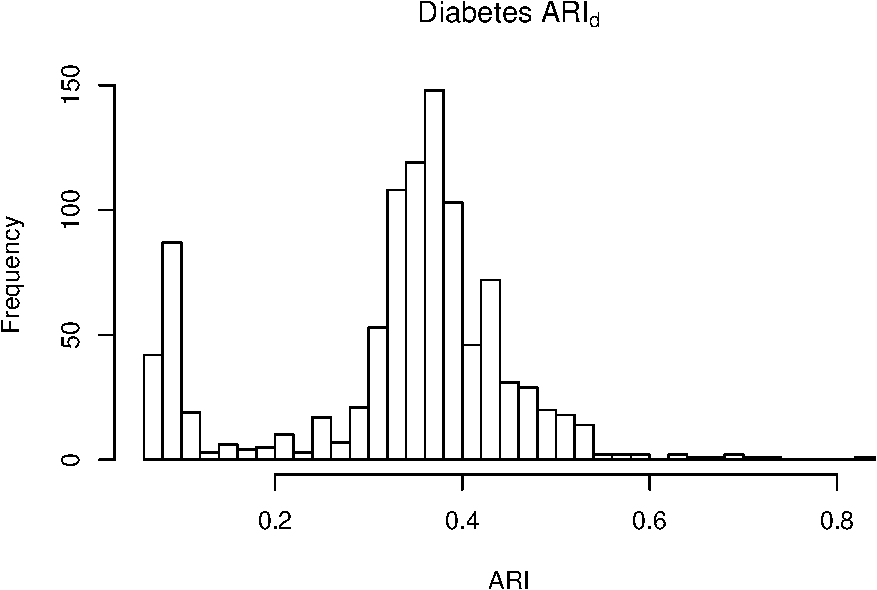
\includegraphics[width=1\linewidth]{Report_files/figure-latex/unnamed-chunk-9-3} \end{center}

\begin{center}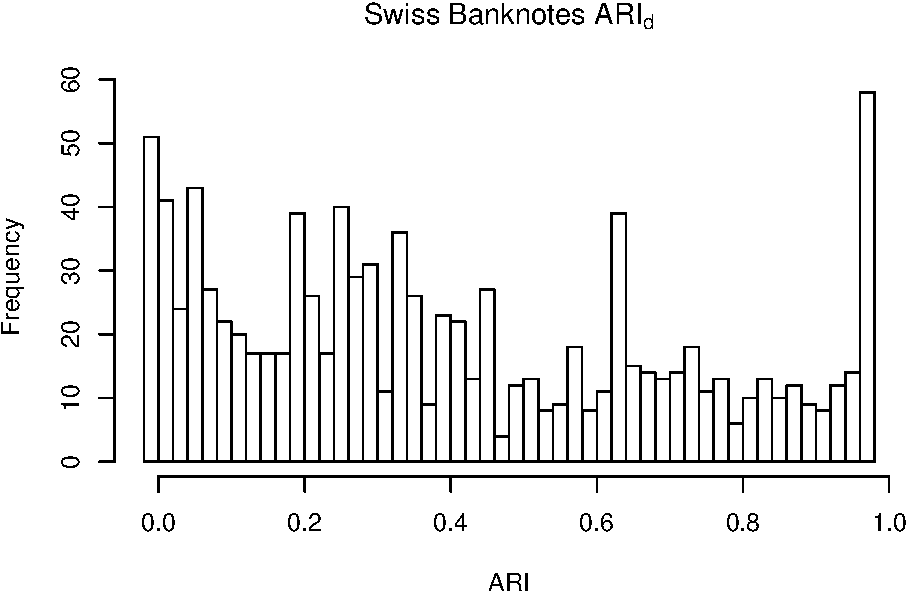
\includegraphics[width=1\linewidth]{Report_files/figure-latex/unnamed-chunk-9-4} \end{center}

\begin{center}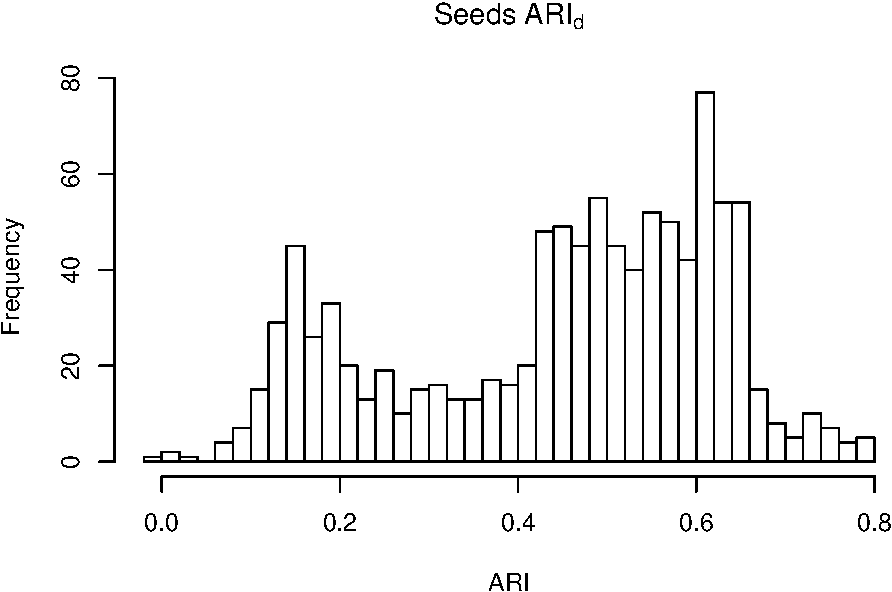
\includegraphics[width=1\linewidth]{Report_files/figure-latex/unnamed-chunk-9-5} \end{center}

\begin{center}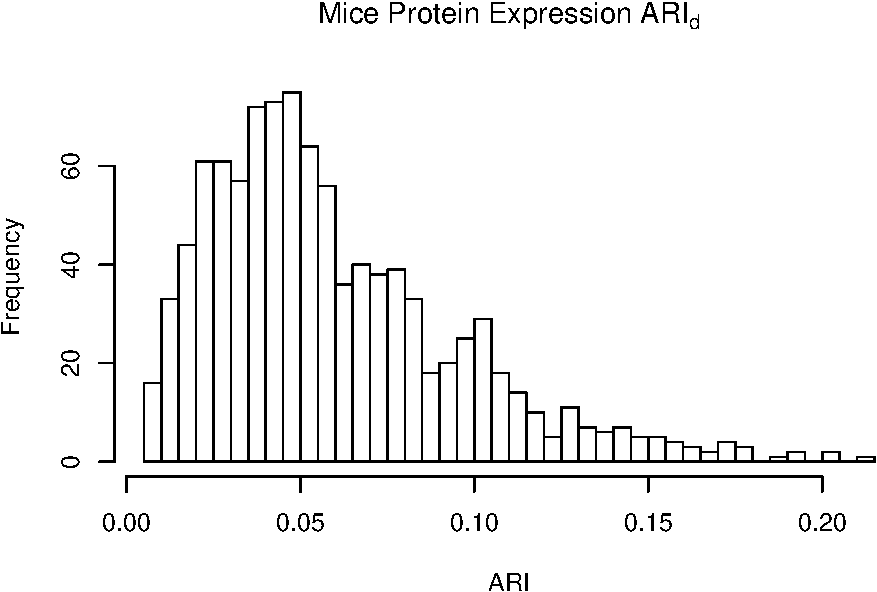
\includegraphics[width=1\linewidth]{Report_files/figure-latex/unnamed-chunk-9-6} \end{center}

\begin{center}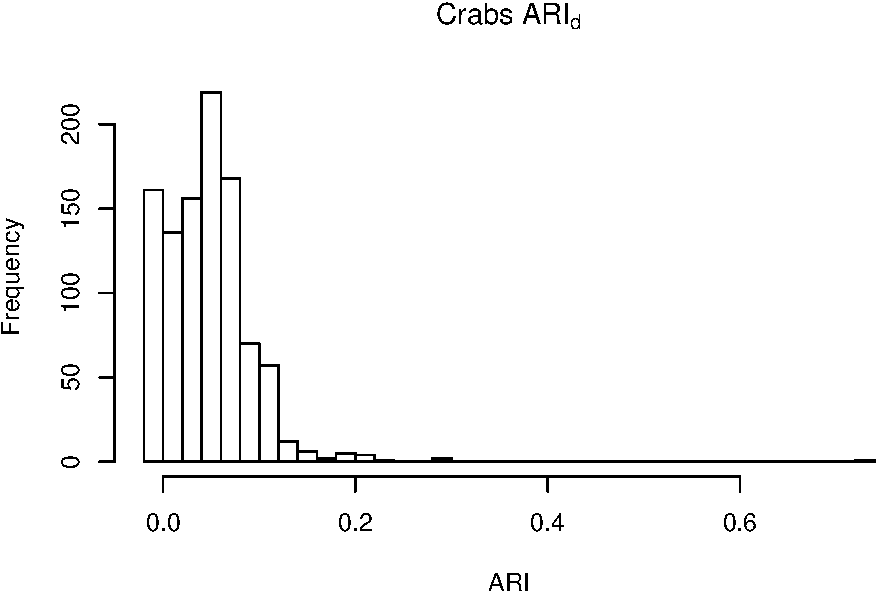
\includegraphics[width=1\linewidth]{Report_files/figure-latex/unnamed-chunk-9-7} \end{center}

\section{\texorpdfstring{For \(\alpha\) = 1, p(reduced dimention) =
3}{For \textbackslash{}alpha = 1, p(reduced dimention) = 3}}\label{for-alpha-1-preduced-dimention-3}

\subsection{Tabel}\label{tabel-2}

\begin{table}[H]
\centering\rowcolors{2}{gray!6}{white}

\begin{tabular}{lrrr}
\hiderowcolors
\toprule
Dataset & ARI\_d & ARI\_p & C\_e\\
\midrule
\showrowcolors
Thyroid & 0.5831656 & 0.3658900 & -22\\
Iris & 0.6201352 & 0.5441285 & -8\\
Diabetes & 0.3801662 & 0.3460760 & -3\\
Swiss Banknotes & 0.8456292 & 0.4330544 & -41\\
Seeds & 0.7732937 & 0.4697687 & -30\\
\addlinespace
Mice Protein Expression & 0.1317362 & 0.0659775 & -7\\
Crabs & 0.0481402 & 0.0452313 & 0\\
\bottomrule
\end{tabular}
\rowcolors{2}{white}{white}
\end{table}

\subsection{Histograms}\label{histograms-3}

\begin{center}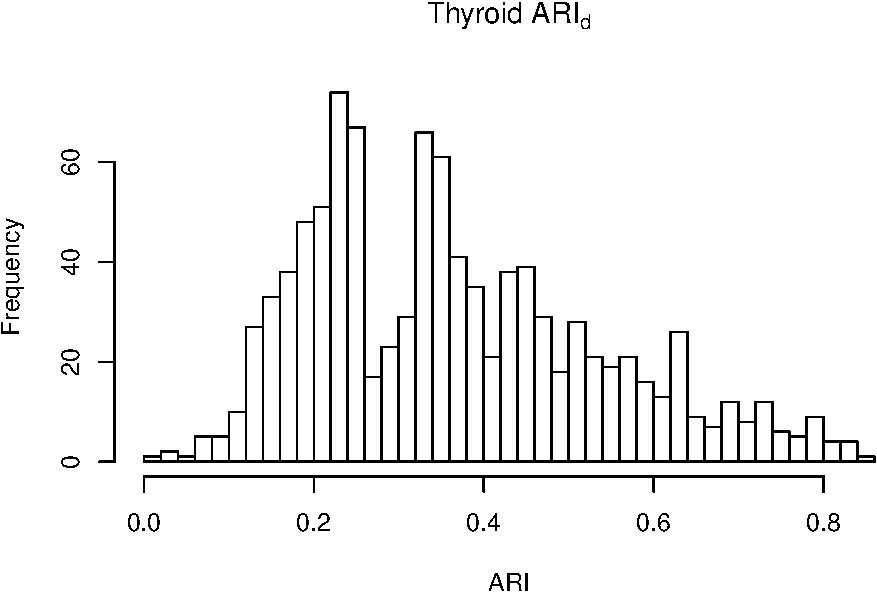
\includegraphics[width=1\linewidth]{Report_files/figure-latex/unnamed-chunk-12-1} \end{center}

\begin{center}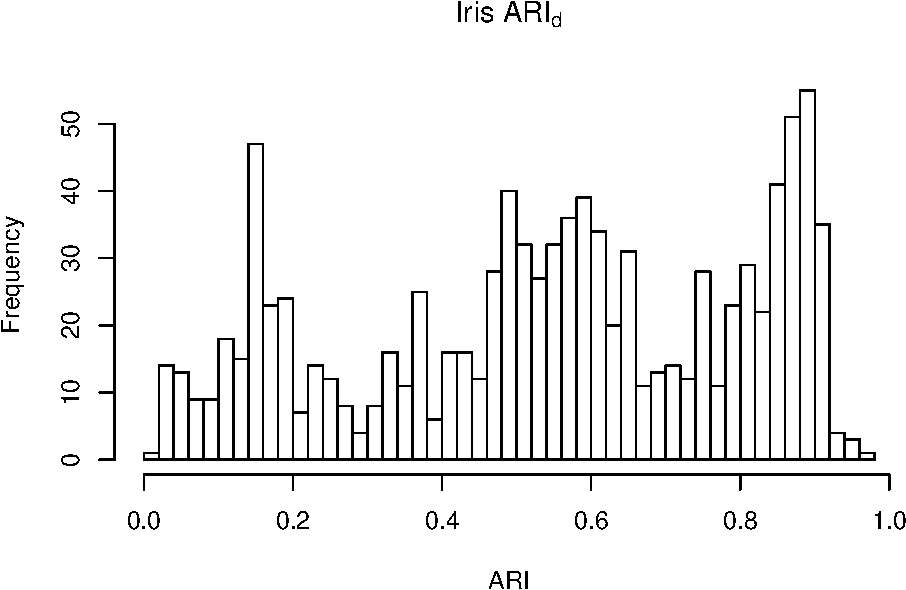
\includegraphics[width=1\linewidth]{Report_files/figure-latex/unnamed-chunk-12-2} \end{center}

\begin{center}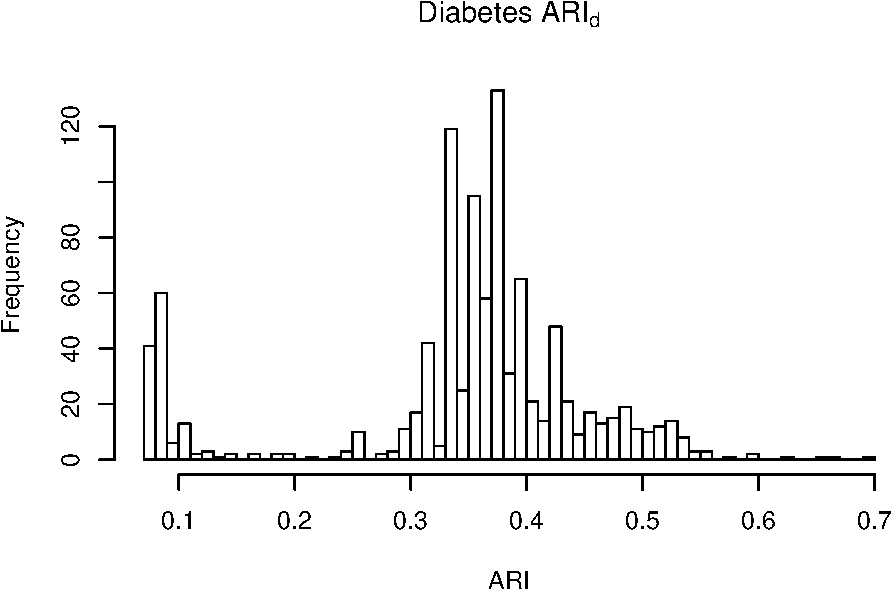
\includegraphics[width=1\linewidth]{Report_files/figure-latex/unnamed-chunk-12-3} \end{center}

\begin{center}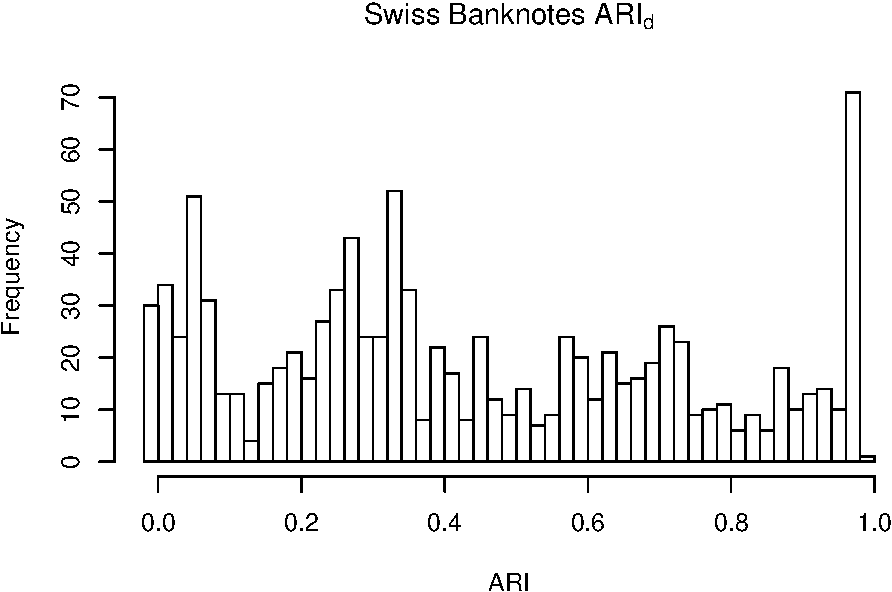
\includegraphics[width=1\linewidth]{Report_files/figure-latex/unnamed-chunk-12-4} \end{center}

\begin{center}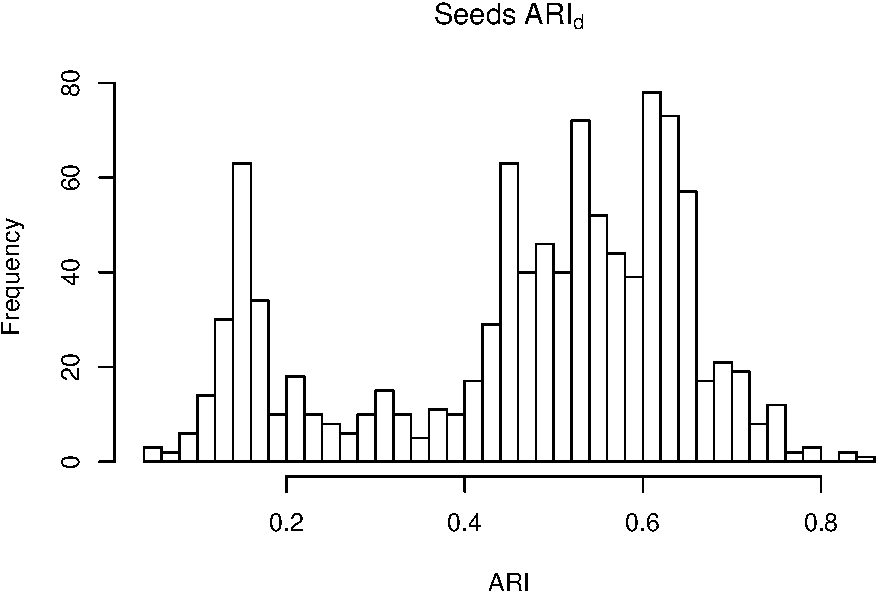
\includegraphics[width=1\linewidth]{Report_files/figure-latex/unnamed-chunk-12-5} \end{center}

\begin{center}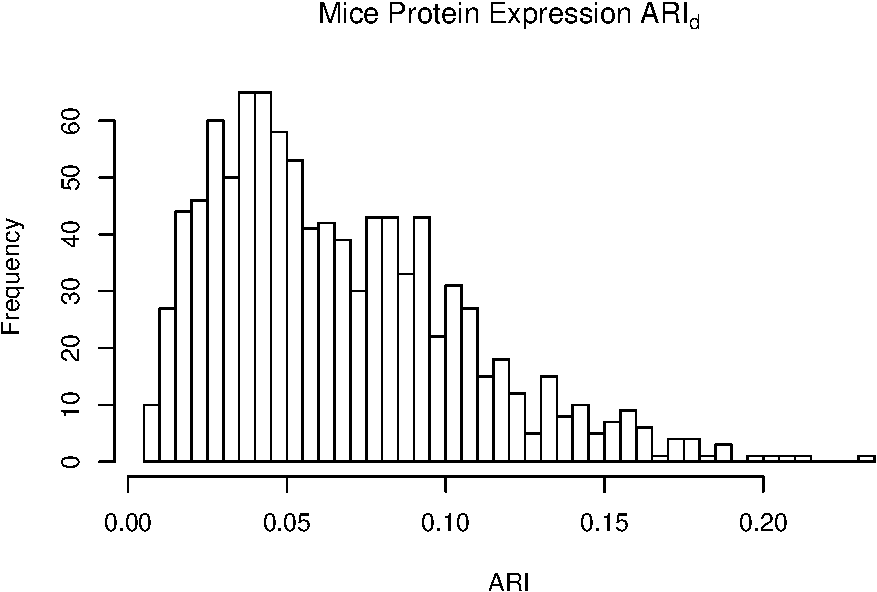
\includegraphics[width=1\linewidth]{Report_files/figure-latex/unnamed-chunk-12-6} \end{center}

\begin{center}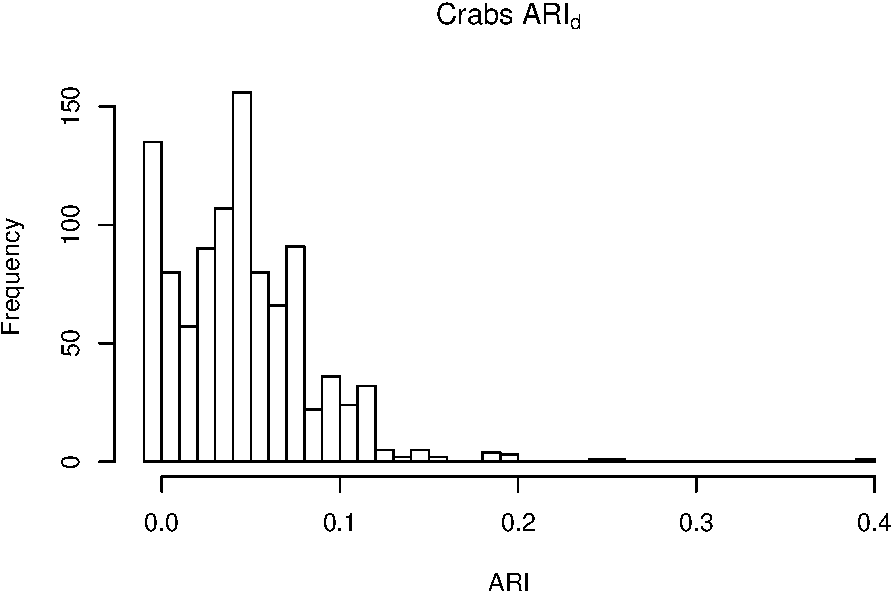
\includegraphics[width=1\linewidth]{Report_files/figure-latex/unnamed-chunk-12-7} \end{center}

\section{\texorpdfstring{For \(s\) = 2, p(reduced dimention) =
2}{For s = 2, p(reduced dimention) = 2}}\label{for-s-2-preduced-dimention-2}

\subsection{Tabel}\label{tabel-3}

\begin{table}[H]
\centering\rowcolors{2}{gray!6}{white}

\begin{tabular}{lrrr}
\hiderowcolors
\toprule
Dataset & ARI\_d & ARI\_p & C\_e\\
\midrule
\showrowcolors
Thyroid & 0.5831656 & 0.4016237 & -18\\
Iris & 0.6201352 & 0.4890477 & -13\\
Diabetes & 0.3801662 & 0.3515435 & -3\\
Swiss Banknotes & 0.8456292 & 0.4012454 & -44\\
Seeds & 0.7732937 & 0.4459104 & -33\\
\addlinespace
Mice Protein Expression & 0.1314435 & 0.0647088 & -7\\
Crabs & 0.0481402 & 0.0467305 & 0\\
\bottomrule
\end{tabular}
\rowcolors{2}{white}{white}
\end{table}

\subsection{Histograms}\label{histograms-4}

\begin{center}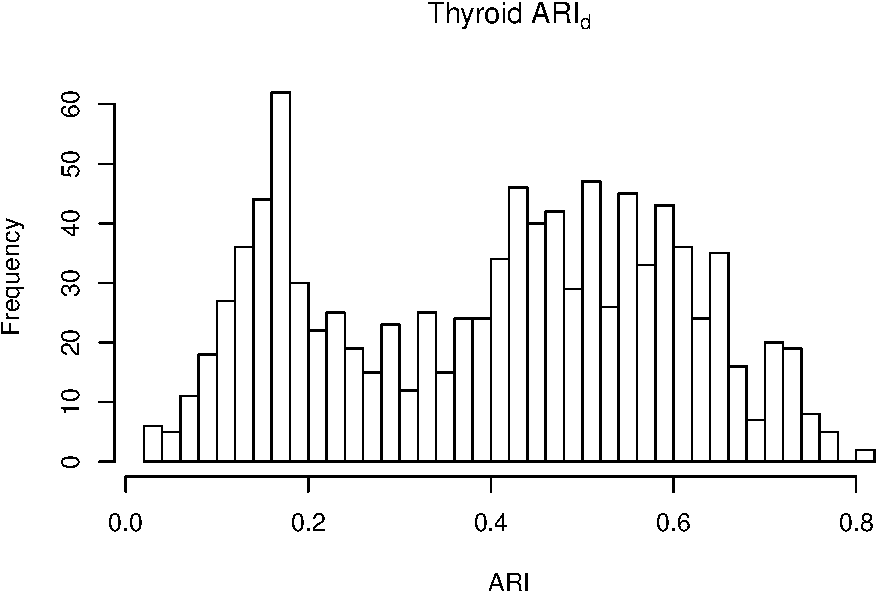
\includegraphics[width=1\linewidth]{Report_files/figure-latex/unnamed-chunk-15-1} \end{center}

\begin{center}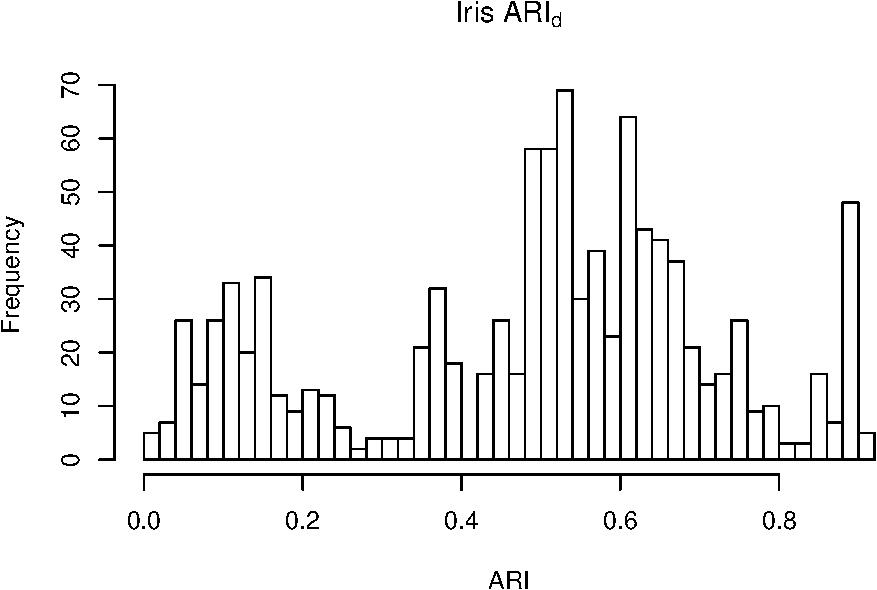
\includegraphics[width=1\linewidth]{Report_files/figure-latex/unnamed-chunk-15-2} \end{center}

\begin{center}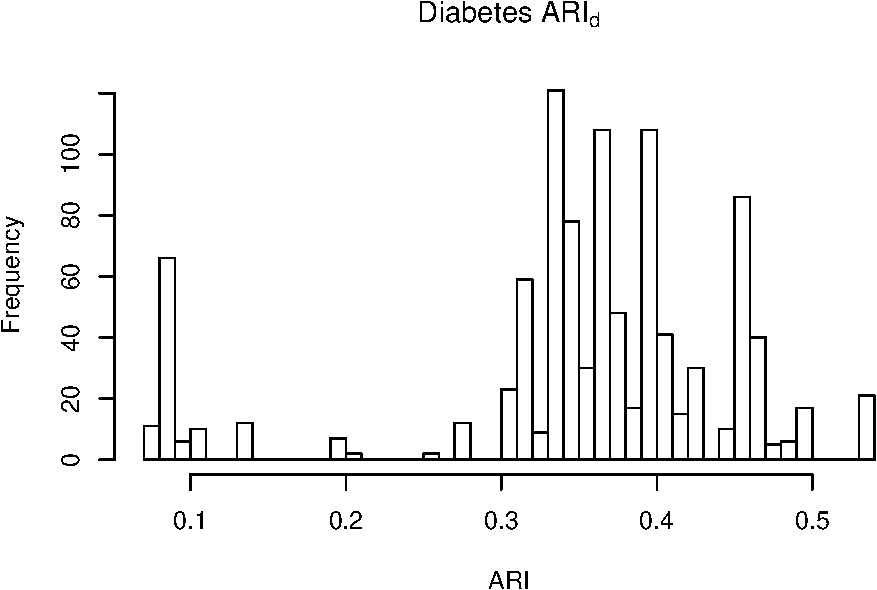
\includegraphics[width=1\linewidth]{Report_files/figure-latex/unnamed-chunk-15-3} \end{center}

\begin{center}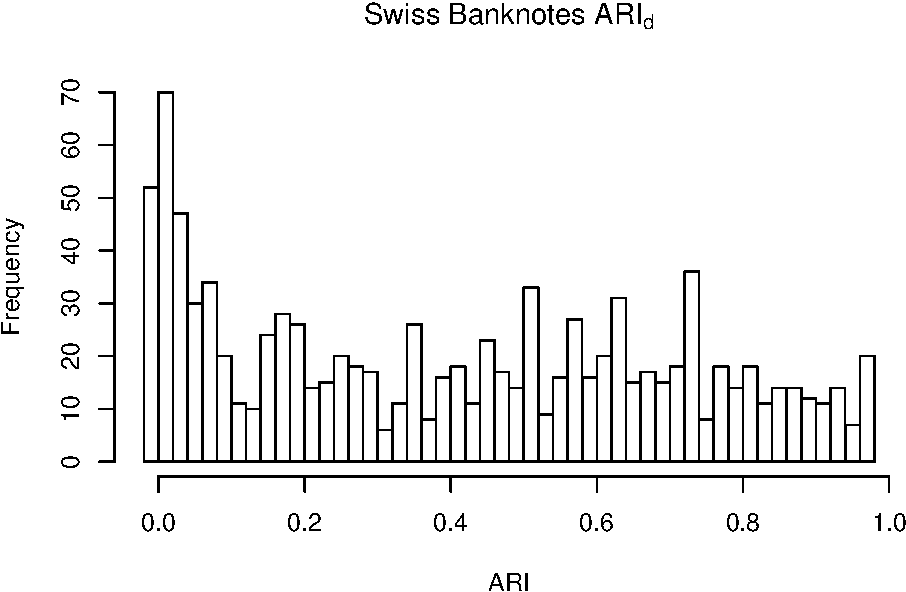
\includegraphics[width=1\linewidth]{Report_files/figure-latex/unnamed-chunk-15-4} \end{center}

\begin{center}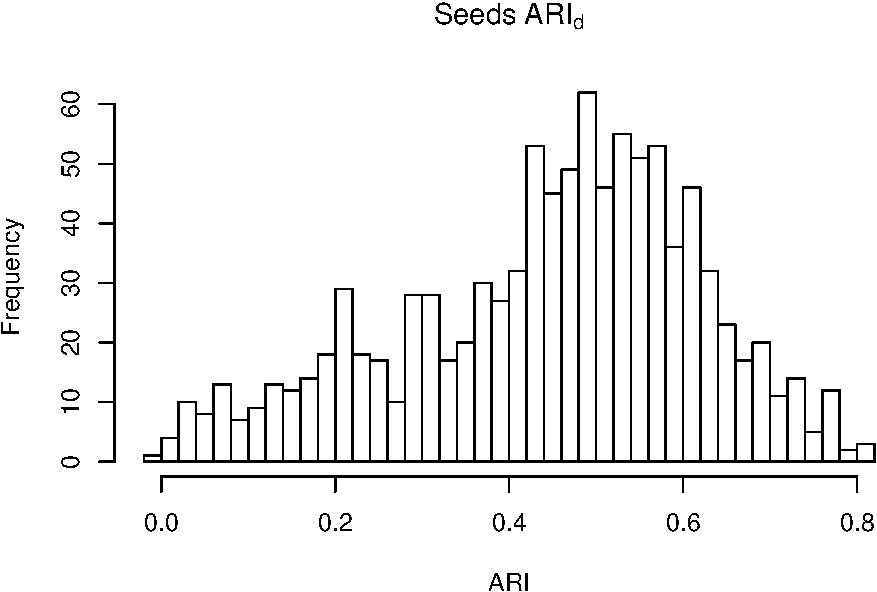
\includegraphics[width=1\linewidth]{Report_files/figure-latex/unnamed-chunk-15-5} \end{center}

\begin{center}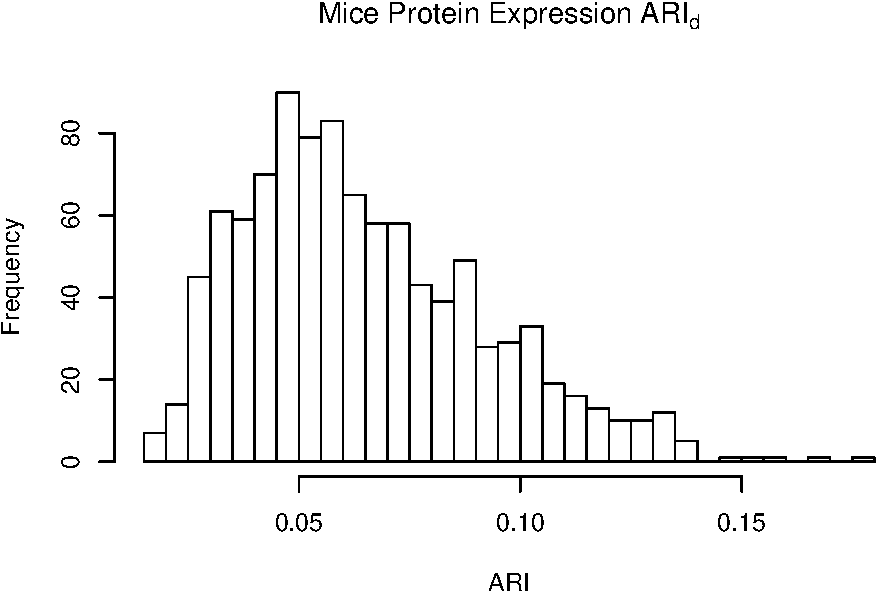
\includegraphics[width=1\linewidth]{Report_files/figure-latex/unnamed-chunk-15-6} \end{center}

\begin{center}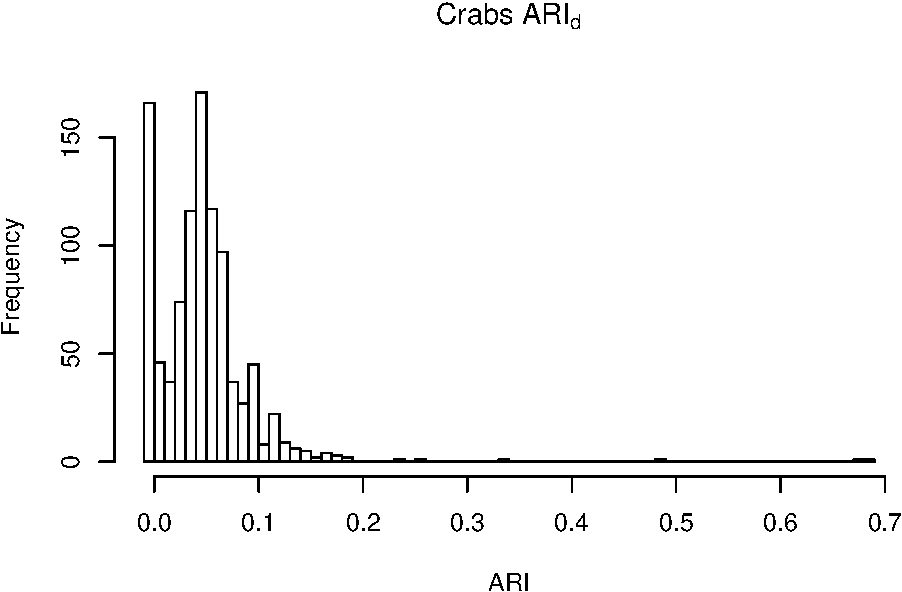
\includegraphics[width=1\linewidth]{Report_files/figure-latex/unnamed-chunk-15-7} \end{center}

\section{\texorpdfstring{For \(s\) = 2, p(reduced dimention) =
2}{For s = 2, p(reduced dimention) = 2}}\label{for-s-2-preduced-dimention-2-1}

\subsection{Tabel}\label{tabel-4}

\begin{table}[H]
\centering\rowcolors{2}{gray!6}{white}

\begin{tabular}{lrrr}
\hiderowcolors
\toprule
Dataset & ARI\_d & ARI\_p & C\_e\\
\midrule
\showrowcolors
Thyroid & 0.5831656 & 0.4386178 & -14\\
Iris & 0.6201352 & 0.5410759 & -8\\
Diabetes & 0.3801662 & 0.3735668 & -1\\
Swiss Banknotes & 0.8456292 & 0.4881694 & -36\\
Seeds & 0.7732937 & 0.5289697 & -24\\
\addlinespace
Mice Protein Expression & 0.1314406 & 0.0798832 & -5\\
Crabs & 0.0481402 & 0.0463655 & 0\\
\bottomrule
\end{tabular}
\rowcolors{2}{white}{white}
\end{table}

\subsection{Histograms}\label{histograms-5}

\begin{center}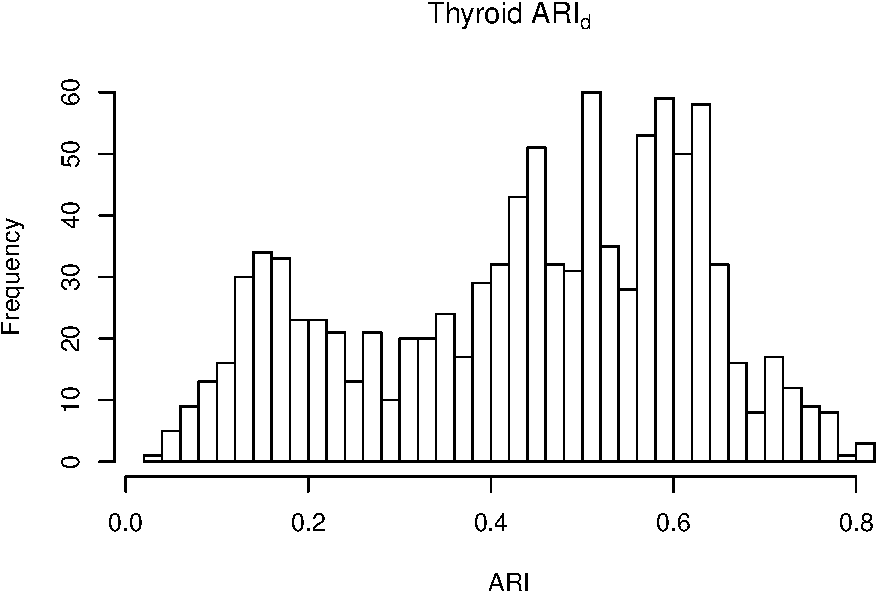
\includegraphics[width=1\linewidth]{Report_files/figure-latex/unnamed-chunk-18-1} \end{center}

\begin{center}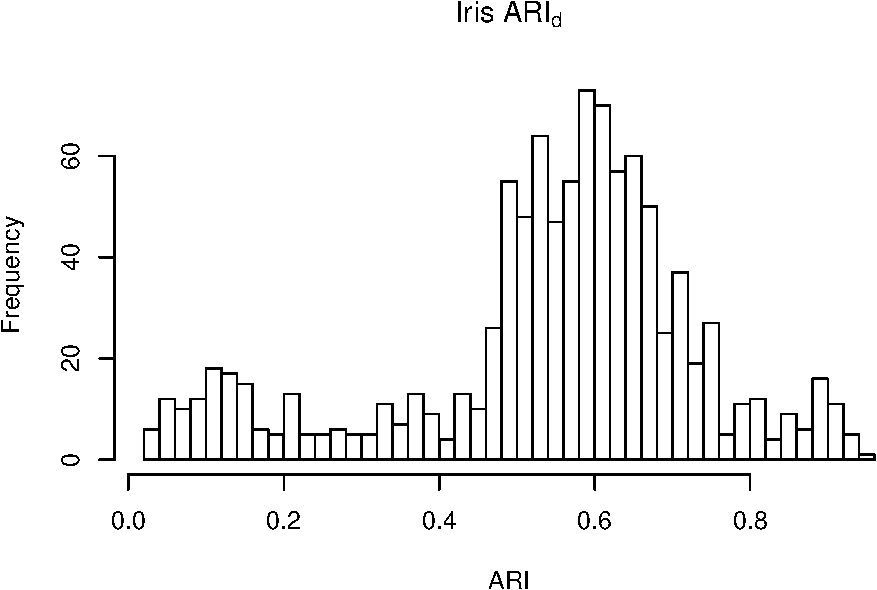
\includegraphics[width=1\linewidth]{Report_files/figure-latex/unnamed-chunk-18-2} \end{center}

\begin{center}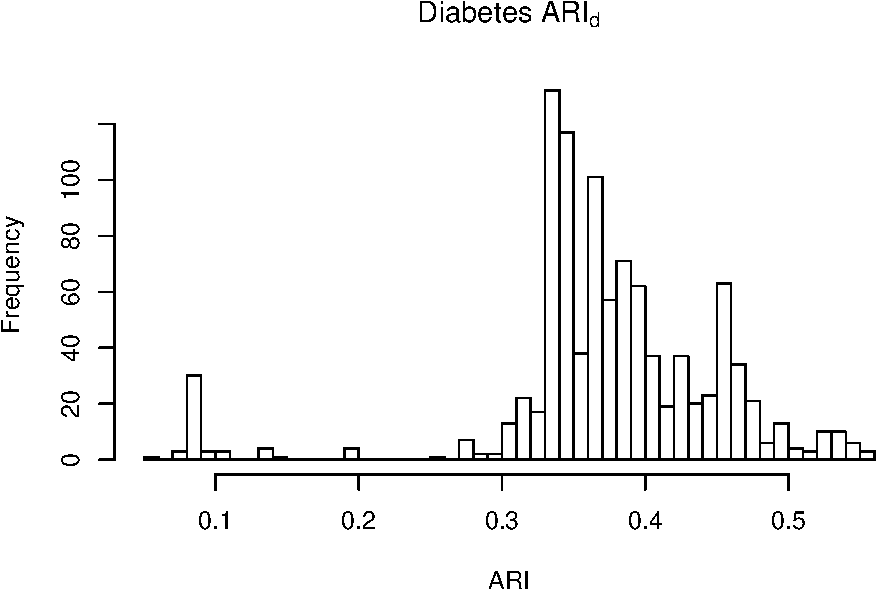
\includegraphics[width=1\linewidth]{Report_files/figure-latex/unnamed-chunk-18-3} \end{center}

\begin{center}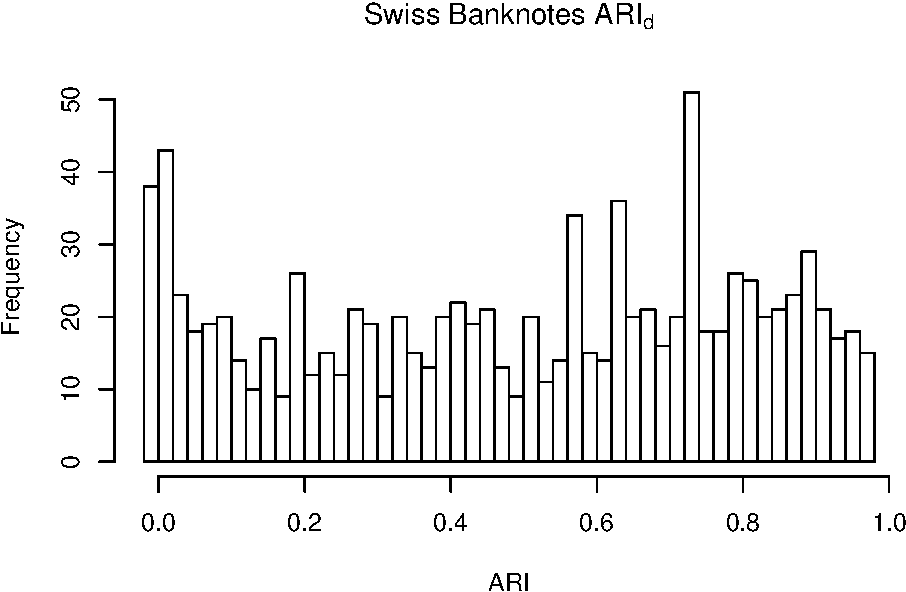
\includegraphics[width=1\linewidth]{Report_files/figure-latex/unnamed-chunk-18-4} \end{center}

\begin{center}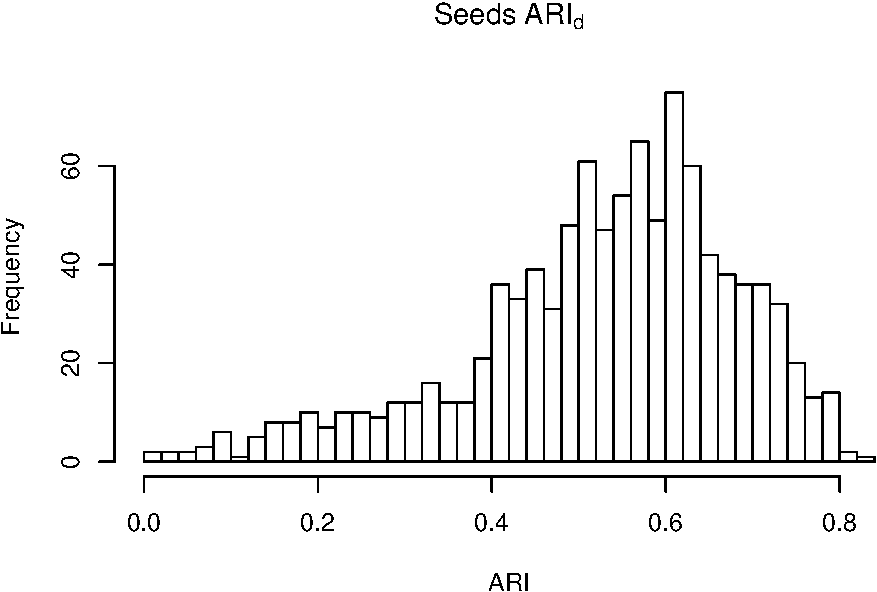
\includegraphics[width=1\linewidth]{Report_files/figure-latex/unnamed-chunk-18-5} \end{center}

\begin{center}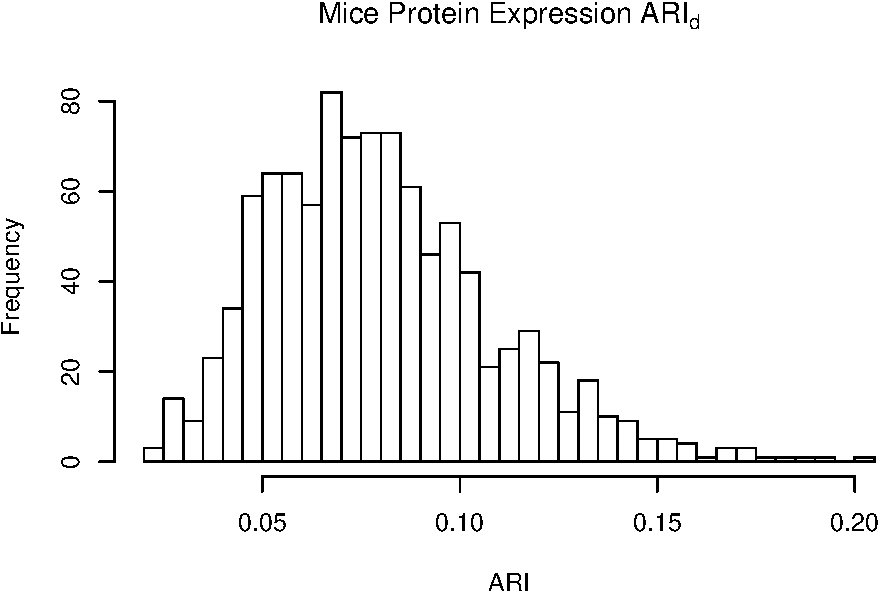
\includegraphics[width=1\linewidth]{Report_files/figure-latex/unnamed-chunk-18-6} \end{center}

\begin{center}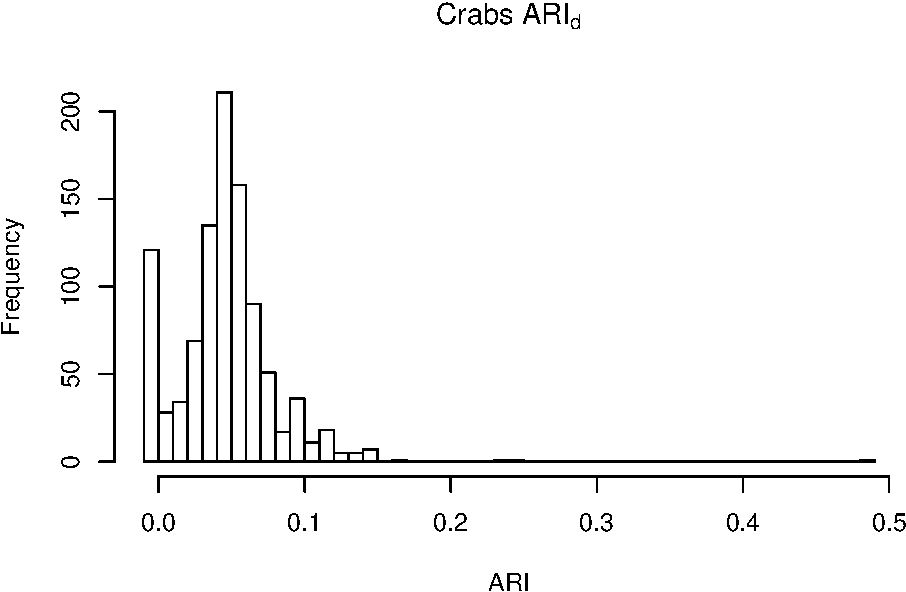
\includegraphics[width=1\linewidth]{Report_files/figure-latex/unnamed-chunk-18-7} \end{center}

\section{For ARI vs alpha, p(reduced dimention) =
2}\label{for-ari-vs-alpha-preduced-dimention-2}

\subsection{Data}\label{data}

\subsection{Plot}\label{plot}

\begin{center}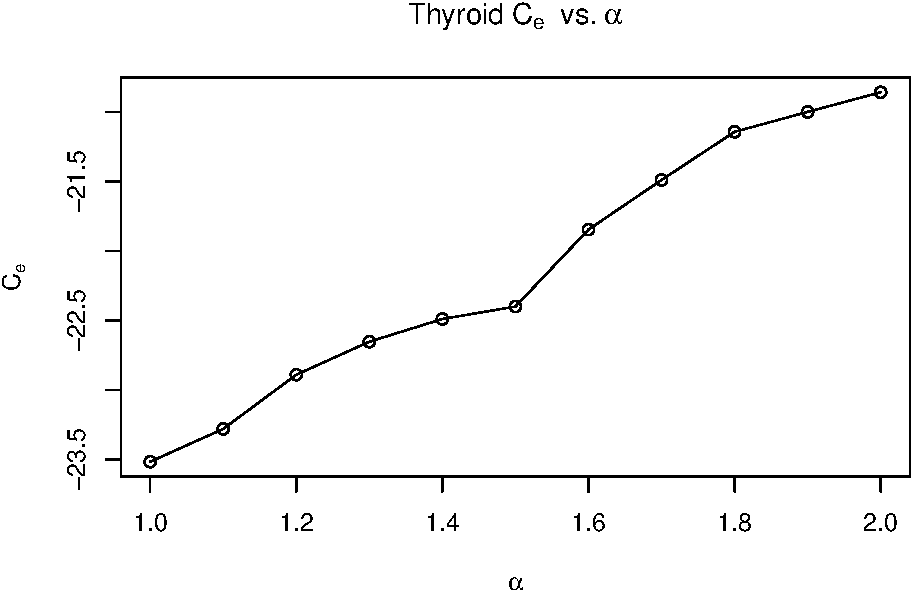
\includegraphics[width=1\linewidth]{Report_files/figure-latex/unnamed-chunk-20-1} \end{center}

\begin{center}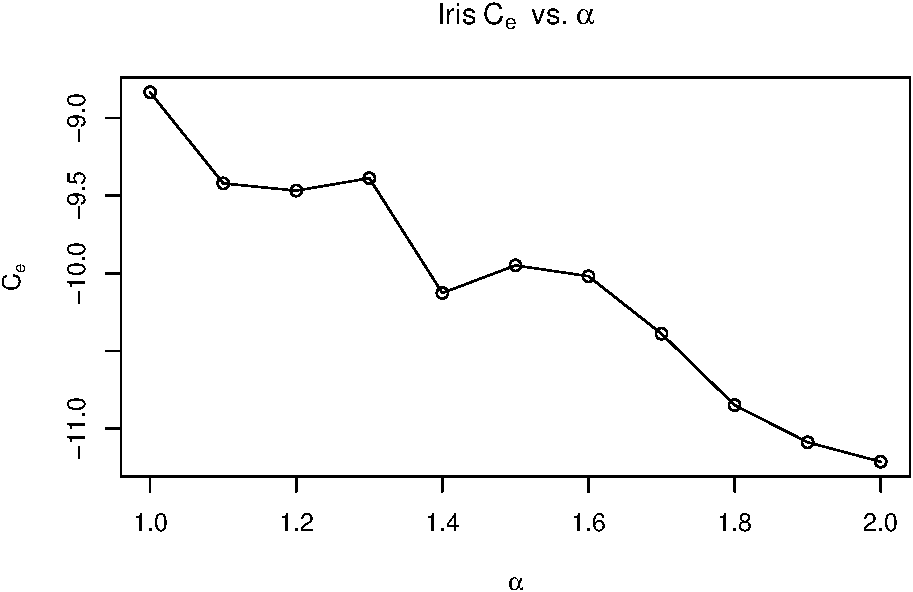
\includegraphics[width=1\linewidth]{Report_files/figure-latex/unnamed-chunk-20-2} \end{center}

\begin{center}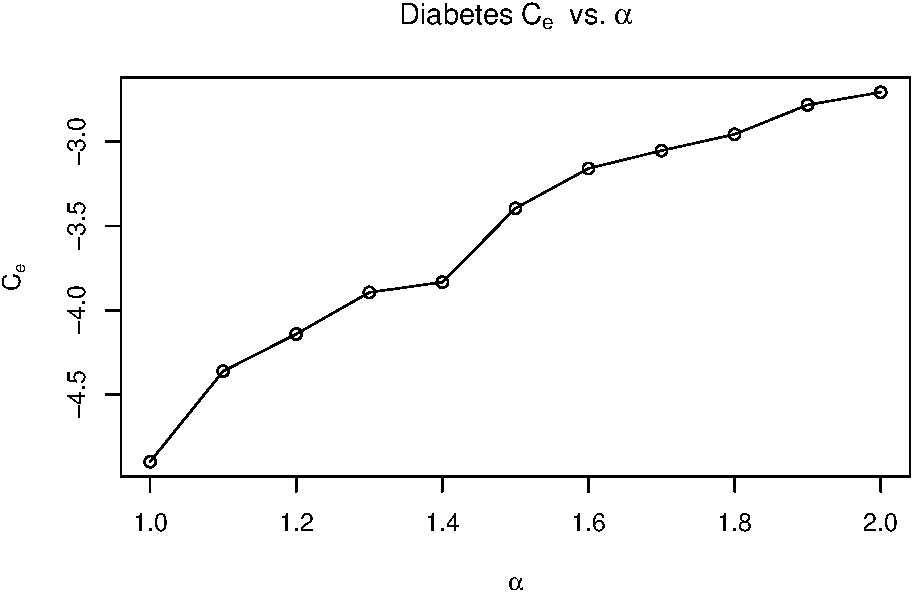
\includegraphics[width=1\linewidth]{Report_files/figure-latex/unnamed-chunk-20-3} \end{center}

\begin{center}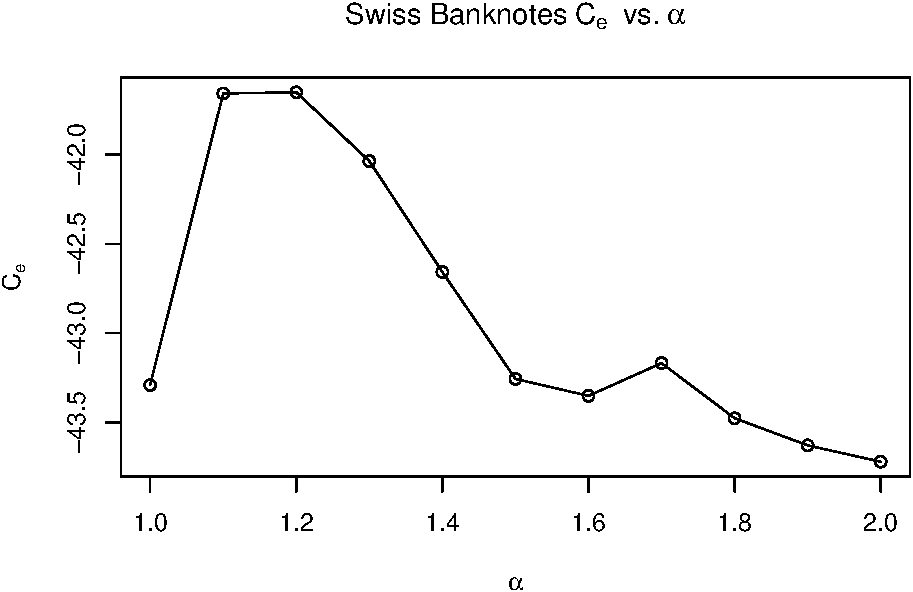
\includegraphics[width=1\linewidth]{Report_files/figure-latex/unnamed-chunk-20-4} \end{center}

\begin{center}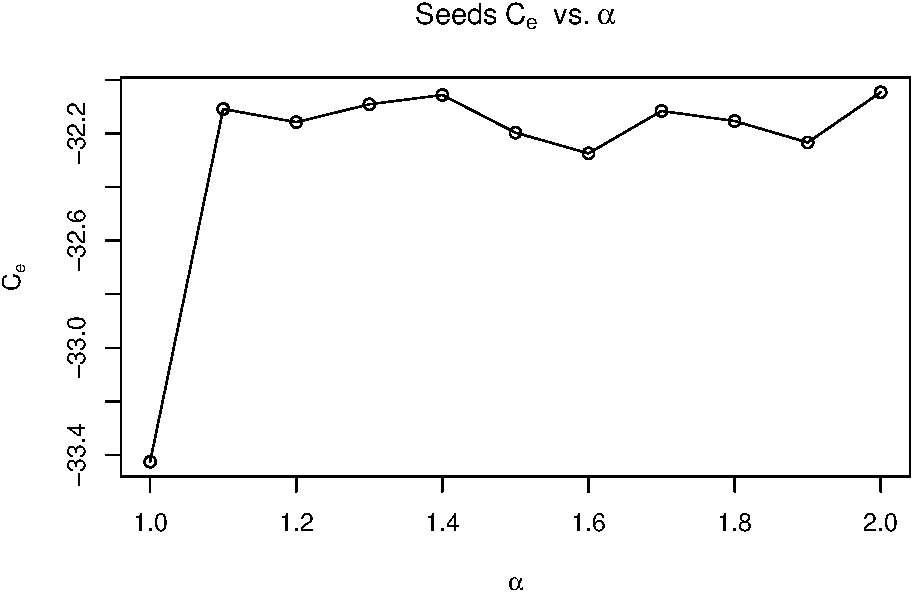
\includegraphics[width=1\linewidth]{Report_files/figure-latex/unnamed-chunk-20-5} \end{center}

\begin{center}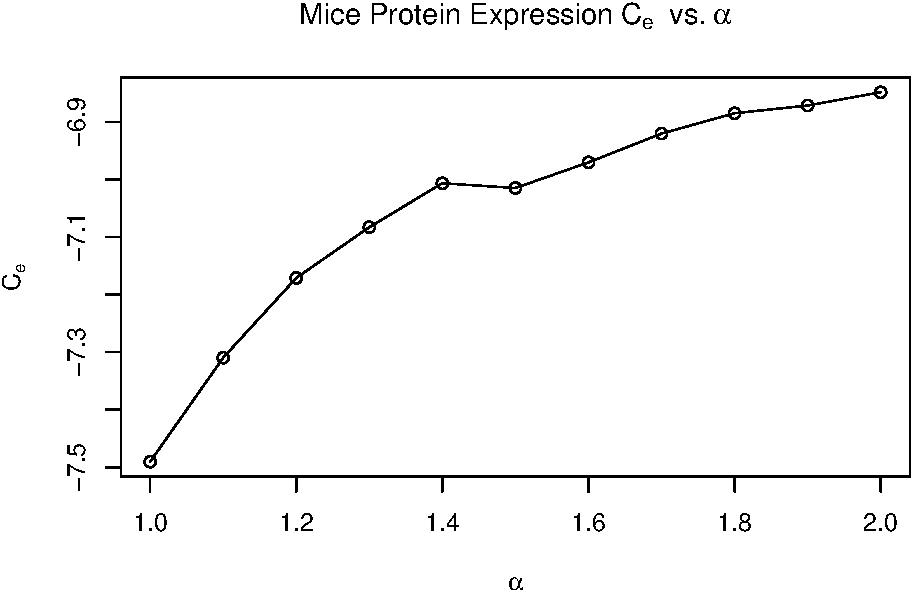
\includegraphics[width=1\linewidth]{Report_files/figure-latex/unnamed-chunk-20-6} \end{center}

\begin{center}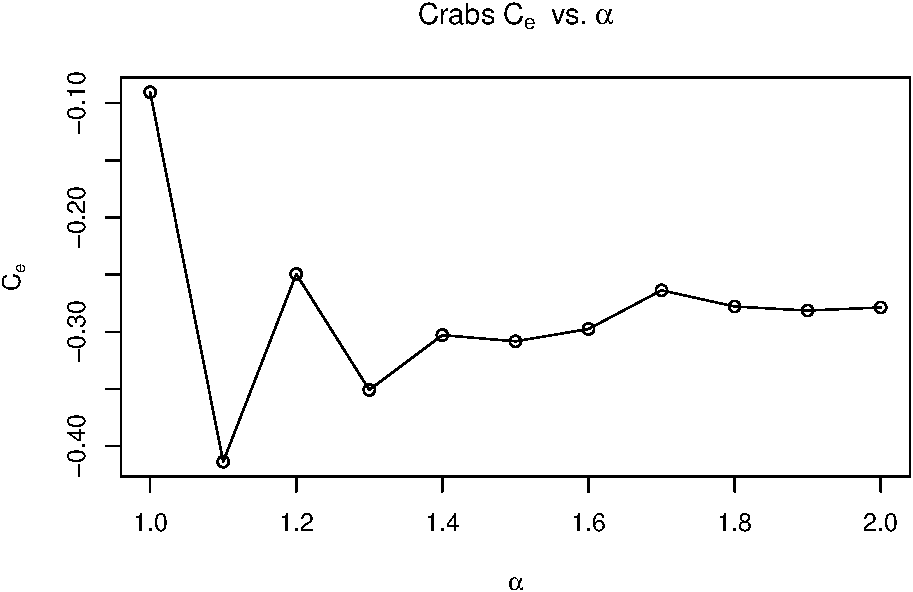
\includegraphics[width=1\linewidth]{Report_files/figure-latex/unnamed-chunk-20-7} \end{center}

\section{For ARI vs alpha, p(reduced dimention) =
3}\label{for-ari-vs-alpha-preduced-dimention-3}

\subsection{Data}\label{data-1}

\subsection{Plot}\label{plot-1}

\begin{center}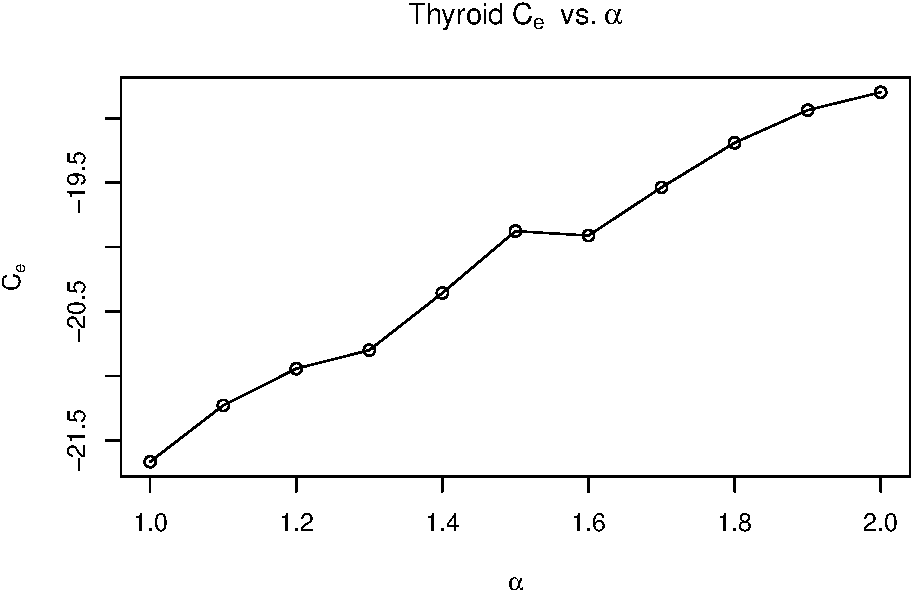
\includegraphics[width=1\linewidth]{Report_files/figure-latex/unnamed-chunk-22-1} \end{center}

\begin{center}\includegraphics[width=1\linewidth]{Report_files/figure-latex/unnamed-chunk-22-2} \end{center}

\begin{center}\includegraphics[width=1\linewidth]{Report_files/figure-latex/unnamed-chunk-22-3} \end{center}

\begin{center}\includegraphics[width=1\linewidth]{Report_files/figure-latex/unnamed-chunk-22-4} \end{center}

\begin{center}\includegraphics[width=1\linewidth]{Report_files/figure-latex/unnamed-chunk-22-5} \end{center}

\begin{center}\includegraphics[width=1\linewidth]{Report_files/figure-latex/unnamed-chunk-22-6} \end{center}

\begin{center}\includegraphics[width=1\linewidth]{Report_files/figure-latex/unnamed-chunk-22-7} \end{center}

\section{For ARI vs s, p(reduced dimention) =
2}\label{for-ari-vs-s-preduced-dimention-2}

\subsection{Data}\label{data-2}

\subsection{Plot}\label{plot-2}

\begin{center}\includegraphics[width=1\linewidth]{Report_files/figure-latex/unnamed-chunk-24-1} \end{center}

\begin{center}\includegraphics[width=1\linewidth]{Report_files/figure-latex/unnamed-chunk-24-2} \end{center}

\begin{center}\includegraphics[width=1\linewidth]{Report_files/figure-latex/unnamed-chunk-24-3} \end{center}

\begin{center}\includegraphics[width=1\linewidth]{Report_files/figure-latex/unnamed-chunk-24-4} \end{center}

\begin{center}\includegraphics[width=1\linewidth]{Report_files/figure-latex/unnamed-chunk-24-5} \end{center}

\begin{center}\includegraphics[width=1\linewidth]{Report_files/figure-latex/unnamed-chunk-24-6} \end{center}

\begin{center}\includegraphics[width=1\linewidth]{Report_files/figure-latex/unnamed-chunk-24-7} \end{center}

\section{For ARI vs s, p(reduced dimention) =
3}\label{for-ari-vs-s-preduced-dimention-3}

\subsection{Data}\label{data-3}

\subsection{Plot}\label{plot-3}

\begin{center}\includegraphics[width=1\linewidth]{Report_files/figure-latex/unnamed-chunk-26-1} \end{center}

\begin{center}\includegraphics[width=1\linewidth]{Report_files/figure-latex/unnamed-chunk-26-2} \end{center}

\begin{center}\includegraphics[width=1\linewidth]{Report_files/figure-latex/unnamed-chunk-26-3} \end{center}

\begin{center}\includegraphics[width=1\linewidth]{Report_files/figure-latex/unnamed-chunk-26-4} \end{center}

\begin{center}\includegraphics[width=1\linewidth]{Report_files/figure-latex/unnamed-chunk-26-5} \end{center}

\begin{center}\includegraphics[width=1\linewidth]{Report_files/figure-latex/unnamed-chunk-26-6} \end{center}

\begin{center}\includegraphics[width=1\linewidth]{Report_files/figure-latex/unnamed-chunk-26-7} \end{center}


\end{document}
